\chapter{Grafos}
\chaplabel{graphs}

%\textbf{Warning to the Reader:} This chapter is still being actively
%developed, meaning that the code has not been thoroughly tested and/or
%the text has not be carefully proofread.

Neste capítulo, estudamos duas representações de grafos e algoritmos básicos que usam essas representações.  

Matematicamente, um \emph{grafo (direcionado)}
\index{grafo}%
\index{grafo direcionado}%
é um par $G=(V,A)$ onde
$V$ é um  conjunto de \emph{vértices}
\index{vertice@vértices}%
e $A$ é um conjunto de pares ordenados
de vértices chamados \emph{arestas}.
\index{aresta}%
Uma aresta #(i,j)# é \emph{direcionado}
\index{vertice@vértice direcionado}%
de #i# para #j#;  #i# é chamado de \emph{fonte}
\index{fonte} da aresta e #j#
é chamado de \emph{alvo}.
\index{alvo}  Um \emph{caminho}%
\index{caminho} em $G$ é uma sequência de
vértices $v_0,\ldots,v_k$ tal que, para cada $i\in\{1,\ldots,k\}$,
a aresta $(v_{i-1},v_{i})$ está em $A$.  Um caminho $v_0,\ldots,v_k$ é um
\emph{ciclo}
\index{ciclo}%
se, além disso, a aresta $(v_k,v_0)$ está em $A$.  Um caminho (ou
ciclo) é \emph{simples}
\index{caminho simples/ciclo}%
se todos os seus vértices forem únicos.  Se houver um caminho de 
algum vértice $v_i$ para algum vértice $v_j$ então nós dizemos que
$v_j$ está ao \emph{alcance}
\index{vertice@vértices ao alcance} de $v_i$.  Um exemplo de grafo é mostrado 
em \figref{graph}.

\begin{figure}
	\begin{center}
		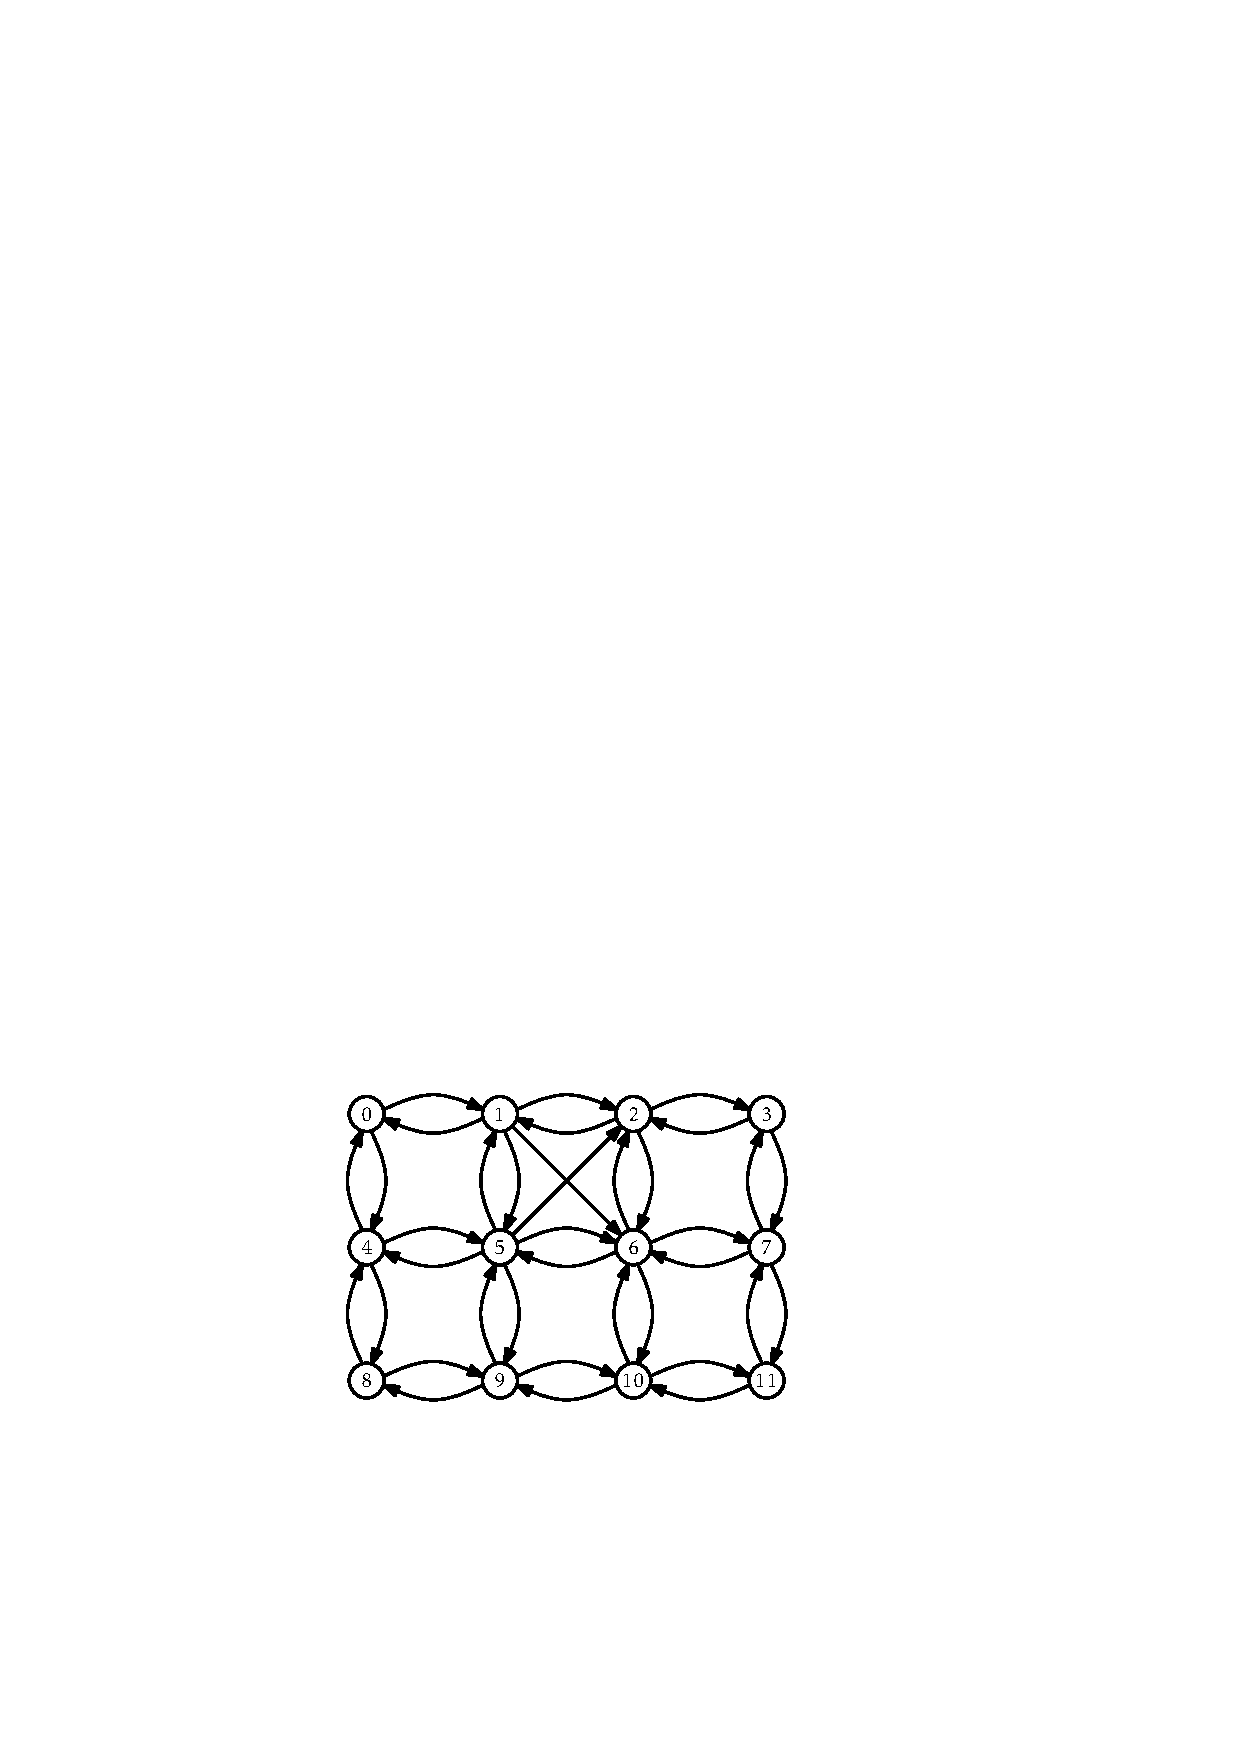
\includegraphics[scale=0.90909]{figs/graph}
	\end{center}
	\caption{Um grafo com doze vértices. Os vértices são desenhados como círculos numerados e as arestas são desenhadas como curvas pontiagudas apontando da origem ao destino.}
	\figlabel{graph}
\end{figure}

Devido à sua capacidade de modelar tantos fenômenos, os grafos têm um enorme número de aplicações. Existem muitos exemplos óbvios. Redes de computadores podem ser modeladas como grafos, com vértices correspondendo a computadores e arestas correspondendo a links de comunicação (direcionados) entre esses computadores. As ruas da cidade podem ser modeladas como grafos, com vértices representando interseções e bordas representando ruas que unem interseções consecutivas.

Exemplos menos óbvios ocorrem assim que percebemos que os grafos podem modelar quaisquer relações de pares dentro de um conjunto. Por exemplo, em um ambiente universitário, podemos ter um \emph{grafo de conflito} de horário
\index{grafo de conflito}%
cujos vértices representam cursos oferecidos na universidade e nos quais a aresta #(i,j)# está presente se e somente se houver pelo menos um aluno que está cursando as aulas #i# e a classe #j#. Assim, uma aresta indica que a prova da classe #i# não deve ser agendado ao mesmo tempo que a prova da classe #j#.

Ao longo desta seção, usaremos #n# para denotar o número de vértices de $G$ e #m# para denotar o número de arestas de $G$. Ou seja, $#n#=|V|$ e $#m#=|A|$. Além disso, assumiremos que $V=\{0,\ldots,#n#-1\}$. Quaisquer outros dados que gostaríamos de associar aos elementos de $V$ podem ser armazenados em um array de comprimento $#n#$.

Algumas operações típicas realizadas em grafos são:
\begin{itemize}
	\item #addEdge(i,j)#: Adicione a aresta $(#i#,#j#)$ a $A$.
	\item #removeEdge(i,j)#: Remova a aresta $(#i#,#j#)$ de $A$.
	\item #hasEdge(i,j)#: Checa se a aresta $(#i#,#j#)\in A$ 
	\item #outEdges(i)#: Retorna uma #List# de todos os inteiros $#j#$ tal que
	$(#i#,#j#)\in A$
	\item #inEdges(i)#: Retorna uma #List# de todos os inteiros $#j#$ tal que
	$(#j#,#i#)\in A$
\end{itemize}

Observe que essas operações não são terrivelmente difíceis de implementar com eficiência. Por exemplo, as três primeiras operações podem ser implementadas diretamente usando um #USet#, para que possam ser implementadas em tempo constante esperado usando as tabelas de hash discutidas no \chapref{hashing}.
As duas últimas operações podem ser implementadas em tempo constante armazenando, para cada vértice, uma lista de seus vértices adjacentes.

No entanto, diferentes aplicativos de grafos têm diferentes requisitos de desempenho para essas operações e, idealmente, podemos usar a implementação mais simples que satisfaça todos os requisitos do aplicativo.
Por esse motivo, discutimos duas grandes categorias de representações gráficas.

\section{#AdjacencyMatrix#: Representando um grafo por uma matriz}
\seclabel{adjacency-matrix}

\index{matriz de adjacência}%
Uma \emph{matriz adjacência} é uma forma de representar um grafo de #n# vértices 
$G=(V,A)$ por uma matriz $#n#\times#n#$, #a#, cujas entradas são valores booleanos.
\codeimport{ods/AdjacencyMatrix.a.n.AdjacencyMatrix(n0)}

A entrada da matriz #a[i][j]# é definido como
\[  #a[i][j]#= 
\begin{cases}
#true# & \text{se $#(i,j)#\in A$} \\
#false# & \text{caso contrário}
\end{cases}
\]
A matriz de adjacência para o grafo da \figref{graph} é mostrada em \figref{graph-adj}.

Nesta representação, as operações #addEdge(i,j)#, #removeEdge(i,j)# e #hasEdge(i,j)# envolvem apenas definir ou ler a entrada da matriz #a[i][j]#:
\codeimport{ods/AdjacencyMatrix.addEdge(i,j).removeEdge(i,j).hasEdge(i,j)}
Essas operações claramente levam um tempo constante por operação.

\begin{figure}
	\begin{center}
		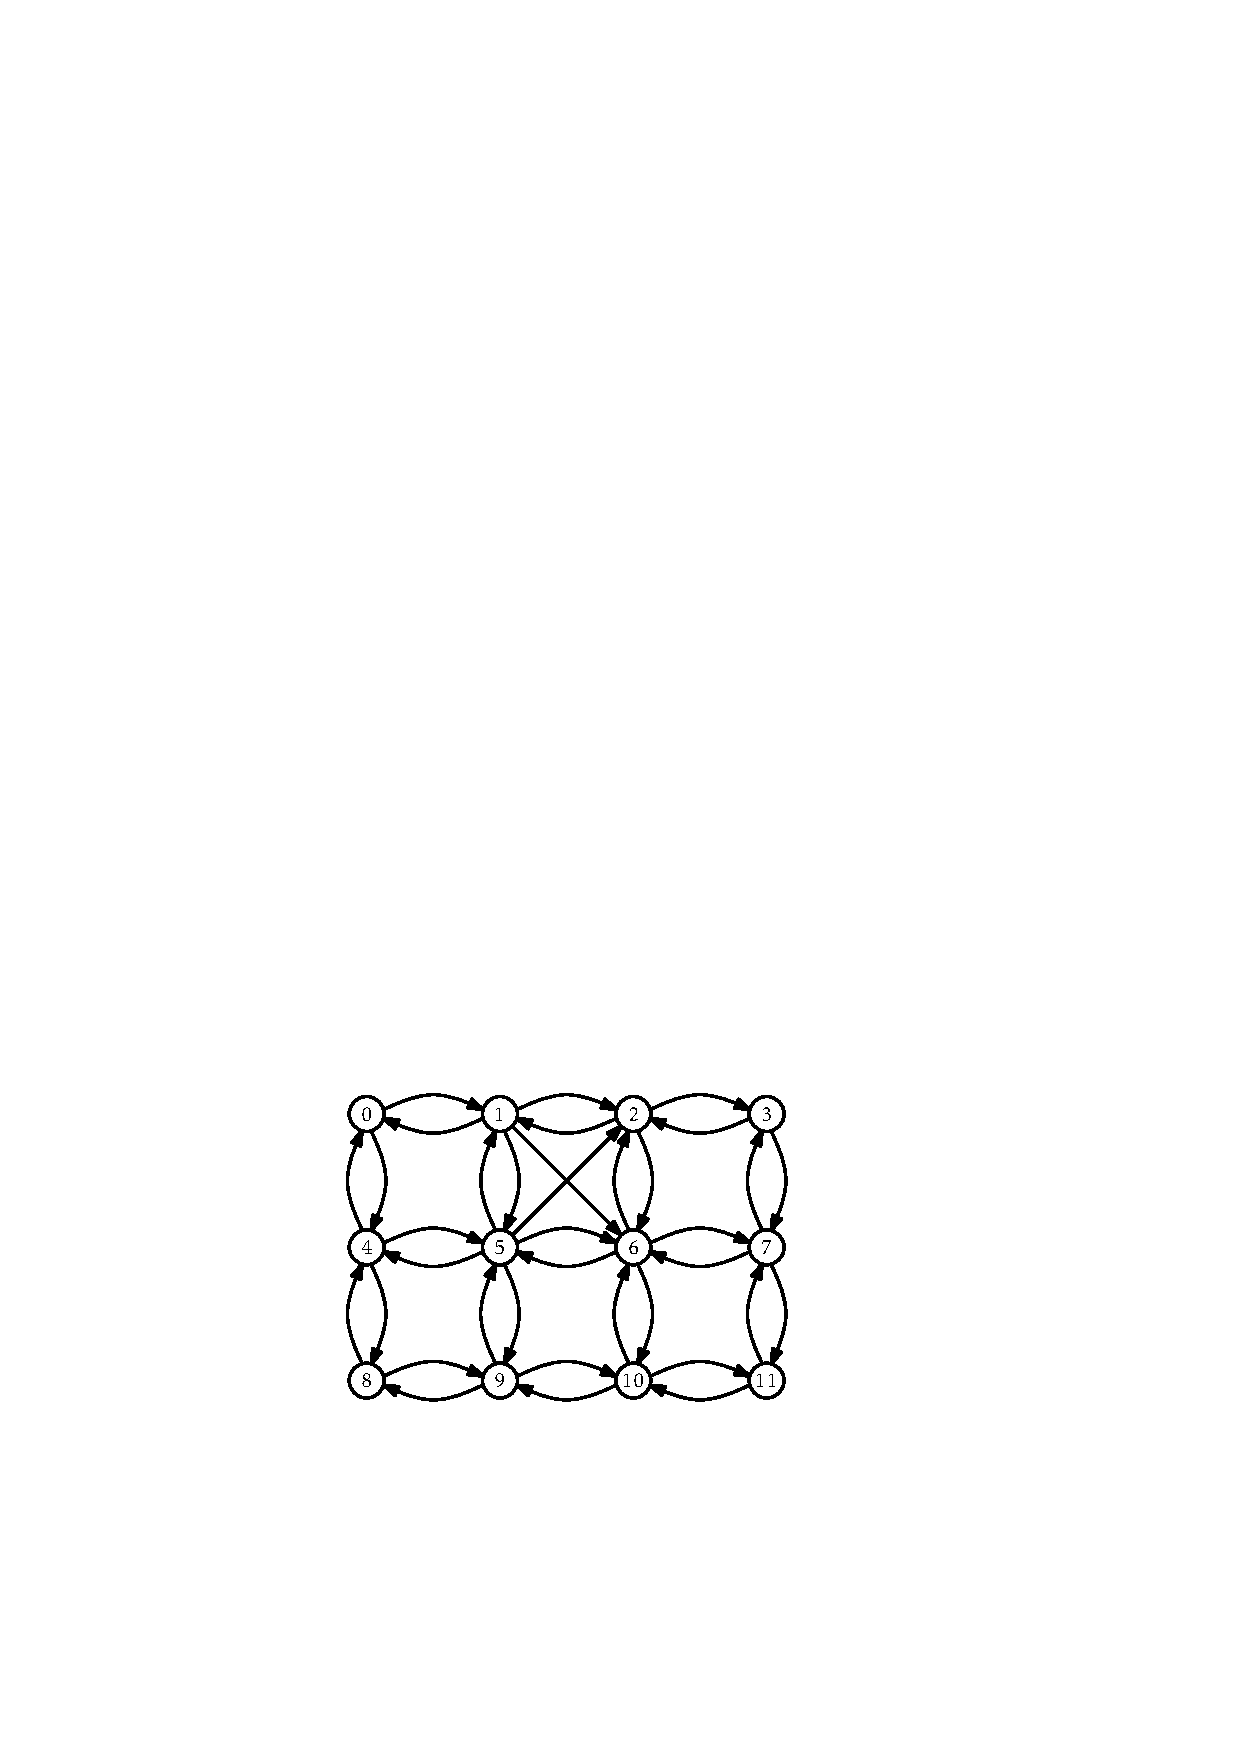
\includegraphics[scale=0.90909]{figs/graph} \\[3ex]
		\begin{tabular}{c|cccccccccccc}
			&0&1&2&3&4&5&6&7&8&9&10&11 \\\hline
			0&0&1&0&0&1&0&0&0&0&0&0 &0\\
			1&1&0&1&0&0&1&1&0&0&0&0 &0\\
			2&1&0&0&1&0&0&1&0&0&0&0 &0\\
			3&0&0&1&0&0&0&0&1&0&0&0 &0\\
			4&1&0&0&0&0&1&0&0&1&0&0 &0\\
			5&0&1&1&0&1&0&1&0&0&1&0 &0\\
			6&0&0&1&0&0&1&0&1&0&0&1 &0\\
			7&0&0&0&1&0&0&1&0&0&0&0 &1\\
			8&0&0&0&0&1&0&0&0&0&1&0 &0\\
			9&0&0&0&0&0&1&0&0&1&0&1 &0\\
			10&0&0&0&0&0&0&1&0&0&1&0 &1\\
			11&0&0&0&0&0&0&0&1&0&0&1 &0\\
		\end{tabular} 
	\end{center}
	\caption{Um grafo e sua matriz de adjacência.}
	\figlabel{graph-adj}
\end{figure}

O desempenho da matriz de adjacência é insatisfatório nas operações #outEdges(i)# e #inEdges(i)#. Para implementá-los, devemos examinar todas as entradas #n# na linha ou coluna correspondente de #a# e reunir todos os índices, #j#, onde #a[i][j]#, respectivamente #a[j][i]#, é verdade.
\javaimport{ods/AdjacencyMatrix.outEdges(i).inEdges(i)}
\cppimport{ods/AdjacencyMatrix.outEdges(i,edges).inEdges(i,edges)}
Essas operações claramente levam tempo por operação $O(#n#)$.  

Outra desvantagem da representação da matriz de adjacência é que ela é grande. Ele armazena uma matriz booleana $#n#\times#n#$, então requer pelo menos $#n#^2$ bits de memória. A implementação aqui usa uma matriz de valores \javaonly{#boolean#}\cpponly{#bool#}\pcodeonly{booleanos}, então ela realmente usa na ordem de $#n#^2$ bytes de memória. Uma implementação mais cuidadosa, que empacote #w# valores booleanos em cada palavra de memória, poderia reduzir esse uso de espaço para $O(#n#^2/#w#)$ palavras de memória.

\begin{thm}
	A estrutura de dados #AdjacencyMatrix# implementa a interface #Graph#.
	Uma #AdjacencyMatrix# suporta as operações
	\begin{itemize}
		\item #addEdge(i,j)#, #removeEdge(i,j)#, e #hasEdge(i,j)# em tempo constante por operação; e
		\item #inEdges(i)#, e #outEdges(i)# em um tempo $O(#n#)$ por operação.
	\end{itemize}
	O espaço usado por uma #AdjacencyMatrix# é  $O(#n#^2)$.
\end{thm}

Apesar de seus altos requisitos de memória e baixo desempenho das operações #inEdges(i)# e #outEdges(i)#, uma #AdjacencyMatrix# ainda pode ser útil para alguns aplicativos. Em particular, quando o grafo $G$ é \emph{denso}, ou seja, tem quase $#n#^2$ arestas, então um uso de memória de $#n#^2$ pode ser aceitável.

A estrutura de dados #AdjacencyMatrix# também é comumente usada porque as operações algébricas na matriz #a# podem ser usadas para calcular com eficiência as propriedades do grafo $G$. Este é um tópico para um curso de algoritmos, mas apontamos uma dessas propriedades aqui: se tratarmos as entradas de #a# como inteiros (1 para #verdadeiro# e 0 para #falso#) e multiplicarmos #a# por si mesmo usando a matriz multiplicação então obtemos a matriz $#a#^2$. Lembre-se, a partir da definição de multiplicação de matrizes, que
\[
#a^2[i][j]# = \sum_{k=0}^{#n#-1} #a[i][k]#\cdot #a[k][j]# \enspace .
\]
Interpretando essa soma em termos do grafo $G$, essa fórmula conta o número de vértices, $#k#$, de forma que $G$ contenha ambas as arestas #(i,k)# e #(k,j)#. Ou seja, ele conta o número de caminhos de $#i#$ a $#j#$ (por meio dos vértices intermediários, $#k#$) cujo comprimento é exatamente dois. Essa observação é a base de um algoritmo que calcula os caminhos mais curtos entre todos os pares de vértices em $G$ usando apenas $O(\log #n#)$ multiplicações de matriz.

\section{#AdjacencyLists#: Um grafo como uma coleção de listas}
\seclabel{adjacency-list}

\index{listas de adjacências}%
As representações com \emph{listas de adjacências} de grafos têm uma abordagem mais centrada no vértice. Existem muitas implementações possíveis de listas de adjacência. Nesta seção, apresentamos uma simples. No final da seção, discutimos diferentes possibilidades. Em uma representação de lista de adjacência, o grafo $G=(V,A)$ é representado como um array, #adj#, de listas. A lista #adj[i]# contém uma lista de todos os vértices adjacentes ao vértice #i#. Ou seja, ele contém todos os índices #j# tais que $#(i,j)#\in A$. 
\codeimport{ods/AdjacencyLists.adj.n.AdjacencyLists(n0)} 
(Um exemplo é mostrado em \figref{graph-adjlist}.) Nesta implementação particular, representamos cada lista em #adj# como \javaonly{um}\cpponly{uma subclasse de} #ArrayStack#, porque gostaríamos de acesso de tempo constante por posição. Outras opções também são possíveis. Especificamente, poderíamos ter implementado #adj# como uma #DLList#.

\begin{figure}
	\begin{center}
		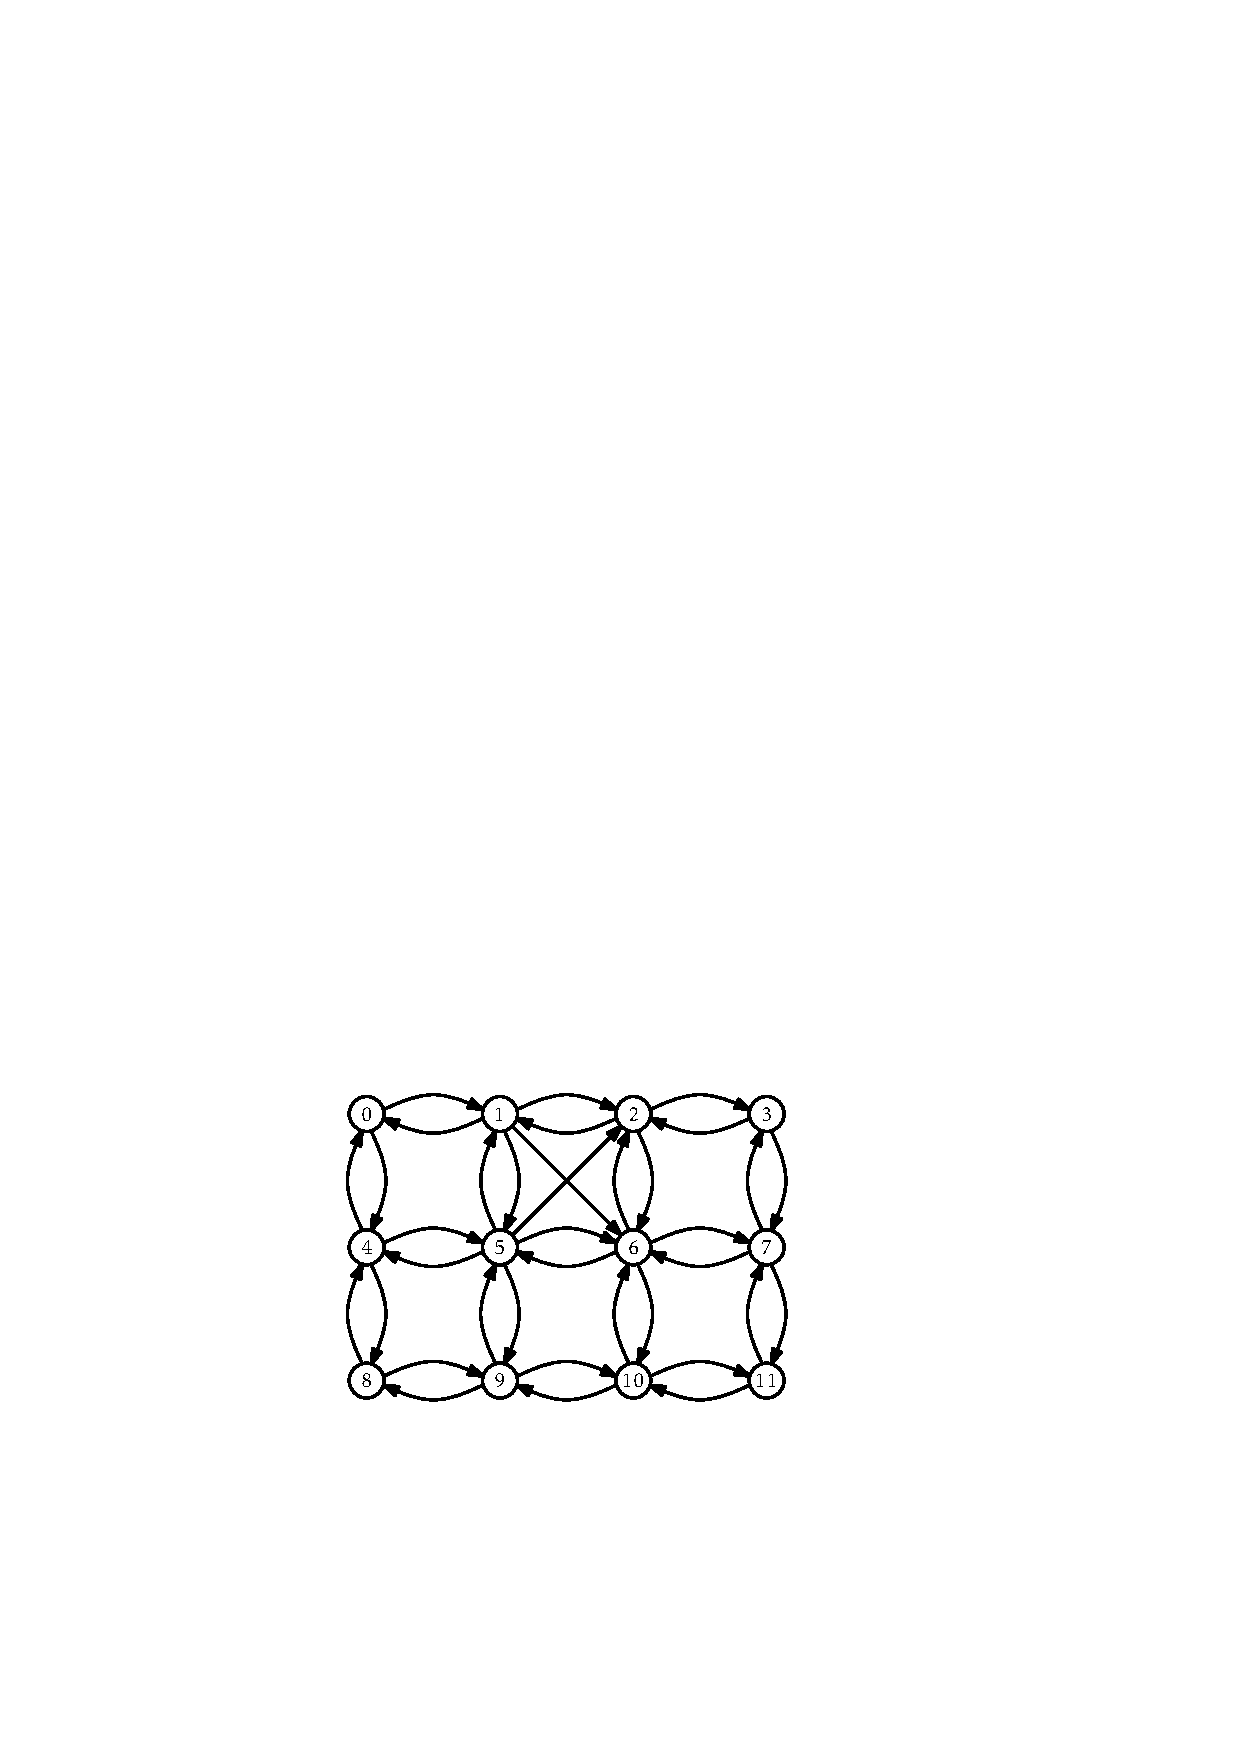
\includegraphics[scale=0.90909]{figs/graph} \\[3ex]
		\begin{tabular}{|c|c|c|c|c|c|c|c|c|c|c|c|c|}\hline
			0&1&2&3&4&5&6 &7 &8&9 &10&11 \\\hline
			1&0&1&2&0&1&5 &6 &4&8 &9 &10 \\
			4&2&3&7&5&2&2 &3 &9&5 &6 &7 \\
			&6&6& &8&6&7 &11& &10&11& \\
			&5& & & &9&10&  & &  &  & \\
			& & & & &4&  &  & &  &  & \\
		\end{tabular} 
	\end{center}
	\caption{Um grafo e suas listas adjacentes}
	\figlabel{graph-adjlist}
\end{figure}


A operação #addEdge(i,j)# apenas acrescenta o valor #j# à lista #adj[i]#:
\codeimport{ods/AdjacencyLists.addEdge(i,j)}
Isso leva um tempo constante.

A operação #removeEdge(i,j)# pesquisa a lista #adj[i]# até encontrar #j# e depois a remove:
\codeimport{ods/AdjacencyLists.removeEdge(i,j)}
Isso leva um tempo $O(\deg(#i#))$, onde $\deg(#i#)$ (o \emph{grau}
\index{grau}%
de $#i#$) conta o número de arestas em $A$ que têm $#i#$ como fonte.

A operação #hasEdge(i,j)# é semelhante; ela pesquisa na lista #adj[i]# até encontrar #j# (e retorna verdadeiro), ou chega ao final da lista (e retorna falso):
\codeimport{ods/AdjacencyLists.hasEdge(i,j)}
Isso também leva tempo $O(\deg(#i#))$.

A operação #outEdges(i)# é muito simples;
\pcodeonly{retorna a lista #adj[i]#}
\javaonly{retorna a lista #adj[i]#}
\cpponly{copia os valores em #adj[i]# para a lista de saída}:
\pcodeimport{ods/AdjacencyLists.outEdges(i)}
\javaimport{ods/AdjacencyLists.outEdges(i)}
\cppimport{ods/AdjacencyLists.outEdges(i,edges)}
\javaonly{Isso claramente leva um tempo constante.}\cpponly{Isso claramente leva um tempo $O(\deg(#i#))$.}

A operação #inEdges(i)# é muito mais trabalhosa. Ele examina cada vértice $j$ verificando se a aresta #(i,j)# existe e, em caso afirmativo, adicionando #j# à lista de saída:
\pcodeimport{ods/AdjacencyLists.inEdges(i)}
\javaimport{ods/AdjacencyLists.inEdges(i)}
\cppimport{ods/AdjacencyLists.inEdges(i,edges)}
Esta operação é muito lenta. Ele faz a varredura da lista de adjacências de cada vértice, portanto, leva tempo $O(#n#+#m#)$.

O teorema a seguir resume o desempenho da estrutura de dados acima:

\begin{thm}
	A estrutura de dados #AdjacencyLists# implementa a interface #Graph#.
	Uma #AdjacencyLists # suporta as operações
	\begin{itemize}
		\item #addEdge(i,j)# em tempo constante por operação;
		\item #removeEdge(i,j)# e #hasEdge(i,j)# em tempo $O(\deg(#i#))$ por operação;
		\javaonly{\item #outEdges(i)# em tempo constante por operação; e}
		\cpponly{\item #outEdges(i)# em tempo $O(\deg(#i#))$ por operação; e}
		\item #inEdges(i)# em tempo $O(#n#+#m#)$ por operação.
	\end{itemize}
	O espaço usado por uma #AdjacencyLists# é  $O(#n#+#m#)$.
\end{thm}

Conforme mencionado anteriormente, existem muitas opções diferentes a serem feitas ao implementar um grafo como uma lista de adjacências. Algumas perguntas que surgem incluem:
\begin{itemize}
	\item Que tipo de coleção deve ser usado para armazenar cada elemento de #adj#? Pode-se usar uma lista baseada em array, uma lista encadeada ou até mesmo uma tabela de hash.
	\item Deve haver uma segunda lista de adjacência, #inadj#, que armazena, para cada #i#, a lista de vértices, #j#, tal que $#(j,i)#\in A$? Isso pode reduzir bastante o tempo de execução da operação #inEdges(i)#, mas requer um pouco mais de trabalho ao adicionar ou remover arestas.
	\item A entrada para a aresta #(i,j)# em #adj[i]# deve ser encadeada por uma referência à entrada correspondente em #inadj[j]#?
	\item As arestas devem ser objetos de primeira classe com seus próprios dados associados? Desta forma, #adj# conteria listas de arestas em vez de listas de vértices (inteiros).
\end{itemize}
A maioria dessas questões se resume a uma troca entre complexidade (e
espaço) de implementação e recursos de desempenho da implementação.

\section{Percurso em Grafos}

Nesta seção, apresentamos dois algoritmos para explorar um grafo, começando em um de seus vértices, #i#, e encontrando todos os vértices que são acessíveis a partir de #i#. Ambos os algoritmos são mais adequados para grafos representados usando uma representação de lista de adjacência. Portanto, ao analisar esses algoritmos, assumiremos que a representação subjacente é uma #AdjacencyLists#.

\subsection{Busca em Largura}

\index{busca em largura}%
O algoritmo \emph{busca em largura} começa em um vértice #i# e visita, primeiro os vizinhos de #i#, depois os vizinhos dos vizinhos de #i#, então os vizinhos dos vizinhos dos vizinhos de #i# e assim por diante.

Este algoritmo é uma generalização do algoritmo de percurso em largura para árvores binárias (\secref{bintree:traversal}) e é muito semelhante; ele usa uma fila, #q#, que inicialmente contém apenas #i#. Em seguida, extrai repetidamente um elemento de #q# e adiciona seus vizinhos a #q#, desde que esses vizinhos nunca tenham estado em #q# antes. A única grande diferença entre o algoritmo de busca por largura para grafos e o algoritmo para árvores é que o algoritmo para grafos deve garantir que não adiciona o mesmo vértice a #q# mais de uma vez. Ele faz isso usando um array booleano auxiliar, #seen#, que rastreia quais vértices já foram descobertos.
\codeimport{ods/Algorithms.bfs(g,r)}
Um exemplo de execução de #bfs(g,0)# no grafo de \figref{graph} é mostrado em \figref{graph-bfs}. Diferentes execuções são possíveis, dependendo da ordem das listas de adjacência; \figref{graph-bfs} usa as listas de adjacência em \figref{graph-adjlist}.

\begin{figure}
	\begin{center}
		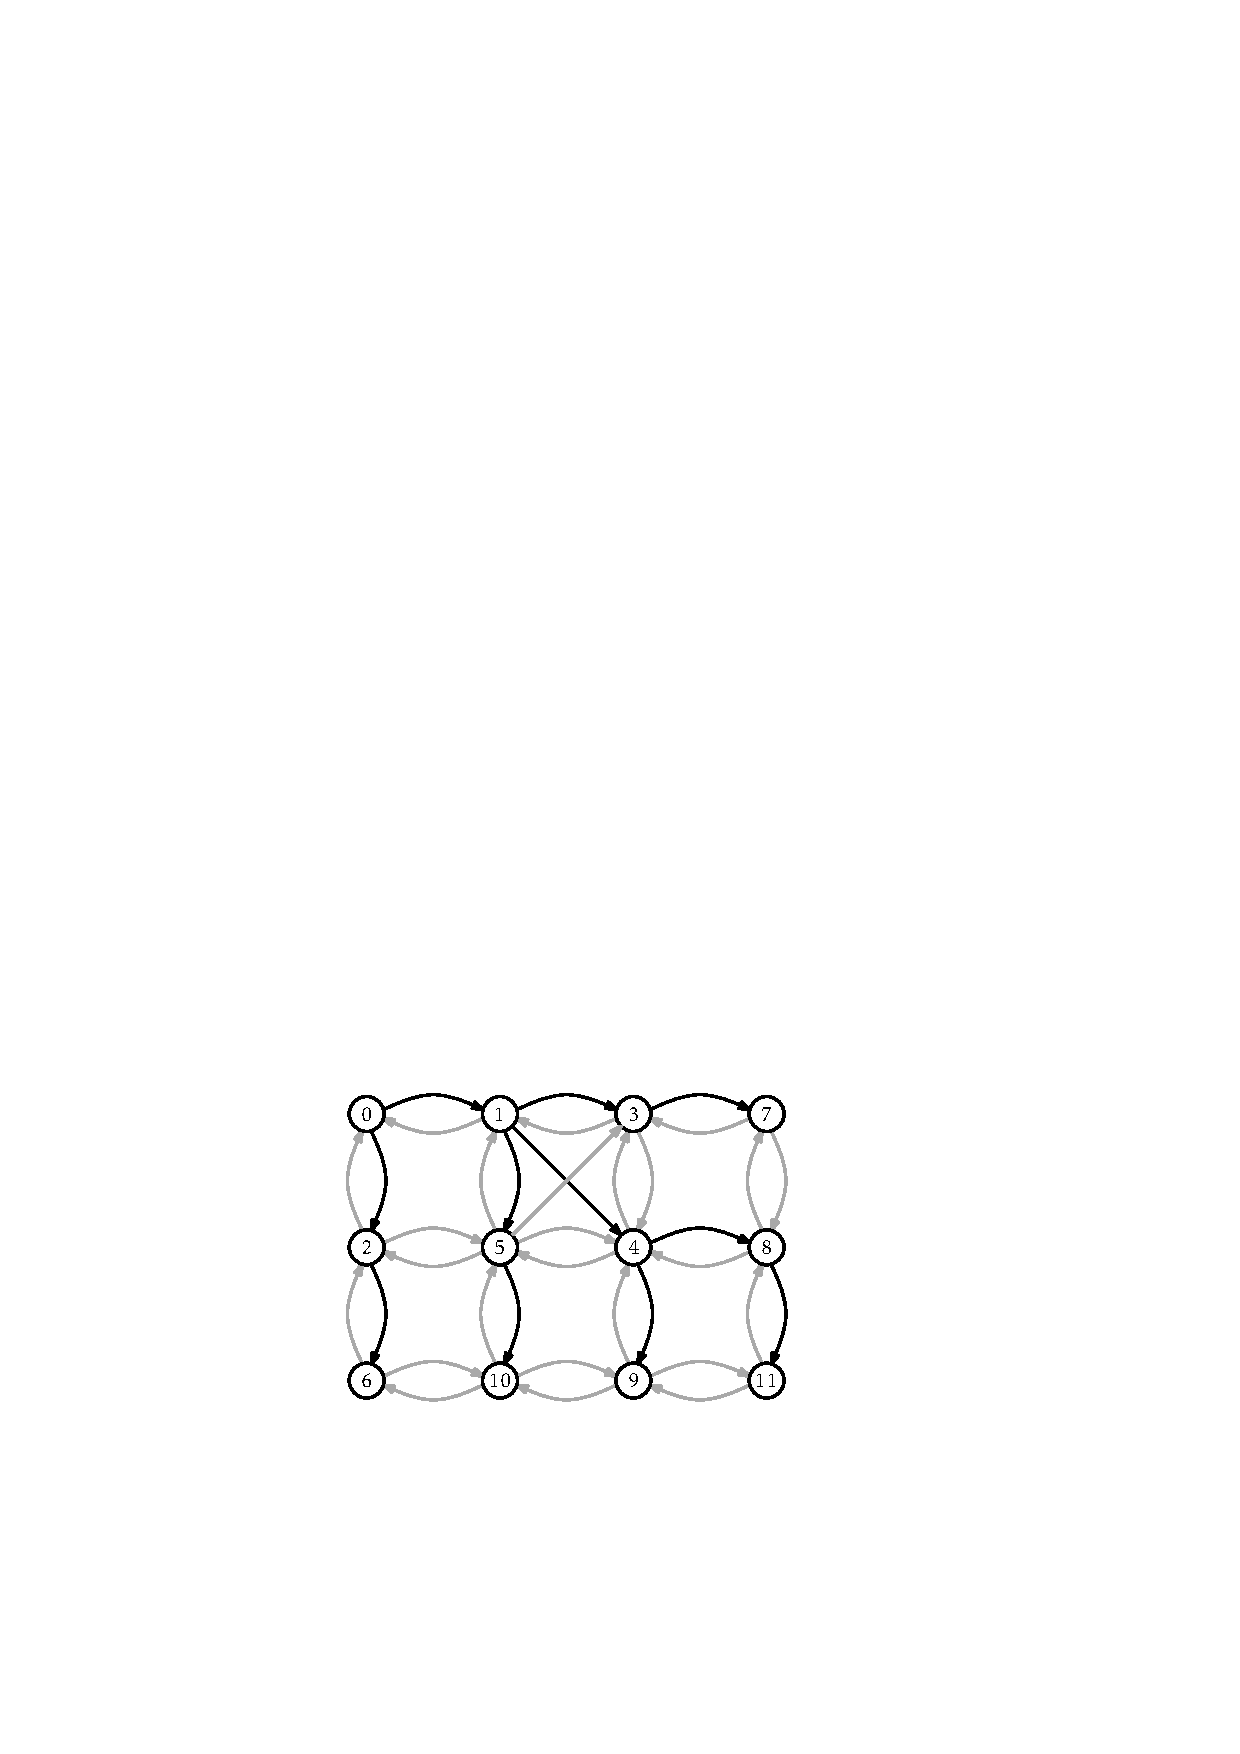
\includegraphics[scale=0.90909]{figs/graph-bfs}
	\end{center}
	\caption[busca em Largura]{Um exemplo de pesquisa em amplitude começando no nó 0. Os nós são rotulados com a ordem em que são adicionados a #q#. As arestas que resultam na adição de nós a #q# são desenhadas em preto, outras arestas são desenhadas em cinza.}
	\figlabel{graph-bfs}
\end{figure}

Analisar o tempo de execução da rotina #bfs(g,i)# é bastante simples. O uso do array #seen# garante que nenhum vértice seja adicionado a #q# mais de uma vez. Adicionar (e posteriormente remover) cada vértice de #q# leva um tempo constante por vértice para um total de $O(#n#)$ tempo. Uma vez que cada vértice é processado pelo laço interno no máximo uma vez, cada lista de adjacência é processada no máximo uma vez, então cada aresta de $G$ é processada no máximo uma vez. Esse processamento, que é feito no loop interno, leva um tempo constante por iteração, para um tempo total de $O(#m#)$. Portanto, todo o algoritmo é executado em tempo $O(#n#+#m#)$.

O teorema a seguir resume o desempenho do algoritmo #bfs(g,r)#.
\begin{thm}\thmlabel{bfs-graph}
	Quando dado como entrada um #Grafo#, #g#, que é implementado usando a estrutura de dados #AdjacencyLists#, o algoritmo #bfs(g,r)# é executado em tempo $O(#n#+#m#)$.
\end{thm}

Uma travessia em largura tem algumas propriedades muito especiais. Chamar #bfs(g,r)# eventualmente enfileirará (e eventualmente removerá da fila) cada vértice #j# de forma que haja um caminho direcionado de #r# para #j#. Além disso, os vértices na distância 0 de #r# (o próprio #r#) entrarão #q# antes dos vértices na distância 1, que entrarão #q# antes dos vértices na distância 2, e assim por diante. Assim, o método #bfs(g,r)# visita vértices em ordem crescente de distância de #r# e vértices que não podem ser alcançados a partir de #r# nunca são visitados.

Uma aplicação particularmente útil do algoritmo de busca por largura é, portanto, na computação de caminhos mais curtos. Para calcular o caminho mais curto de #r# para todos os outros vértices, usamos uma variante de #bfs(g,r)# que usa uma matriz auxiliar, #p#, de comprimento #n#. Quando um novo vértice #j# é adicionado a #q#, definimos #p[j]=i#. Desta forma, #p[j]# se torna o penúltimo nó em um caminho mais curto de #r# a #j#. Repetindo isso, tomando #p[p[j]#, #p[p[p[j]]]#, e assim por diante, podemos reconstruir o (reverso de) um caminho mais curto de #r# para #j#.


\subsection{Pesquisa em profundidade}

O algoritmo \emph{Pesquisa em profundidade}
\index{Pesquisa em profundidade}%
é semelhante ao algoritmo padrão para percorrer árvores binárias;
ele primeiro explora completamente uma subárvore antes de retornar ao nó atual e, em seguida, explorar a outra subárvore. Outra maneira de pensar na pesquisa em profundidade é dizer que ela é semelhante à pesquisa em largura, exceto que usa uma pilha em vez de uma fila.

Durante a execução do algoritmo de pesquisa em profundidade, cada vértice, #i#, recebe uma cor, #c[i]#: #branco# se nunca vimos o vértice antes, #cinza# se estivermos atualmente visitando aquele vértice, e #preto# se terminarmos de visitar aquele vértice. A maneira mais fácil de pensar na pesquisa em profundidade é como um algoritmo recursivo. Ele começa visitando #r#. Ao visitar um vértice #i#, primeiro marcamos #i# como #cinza#. Em seguida, varremos a lista de adjacências de #i# e visitamos recursivamente qualquer vértice branco que encontrarmos nesta lista. Finalmente, terminamos o processamento #i#, então colorimos #i# de preto e retornamos.
\codeimport{ods/Algorithms.dfs(g,r).dfs(g,i,c)}
Um exemplo da execução deste algoritmo é mostrado em \figref{graph-dfs}.

\begin{figure}
	\begin{center}
		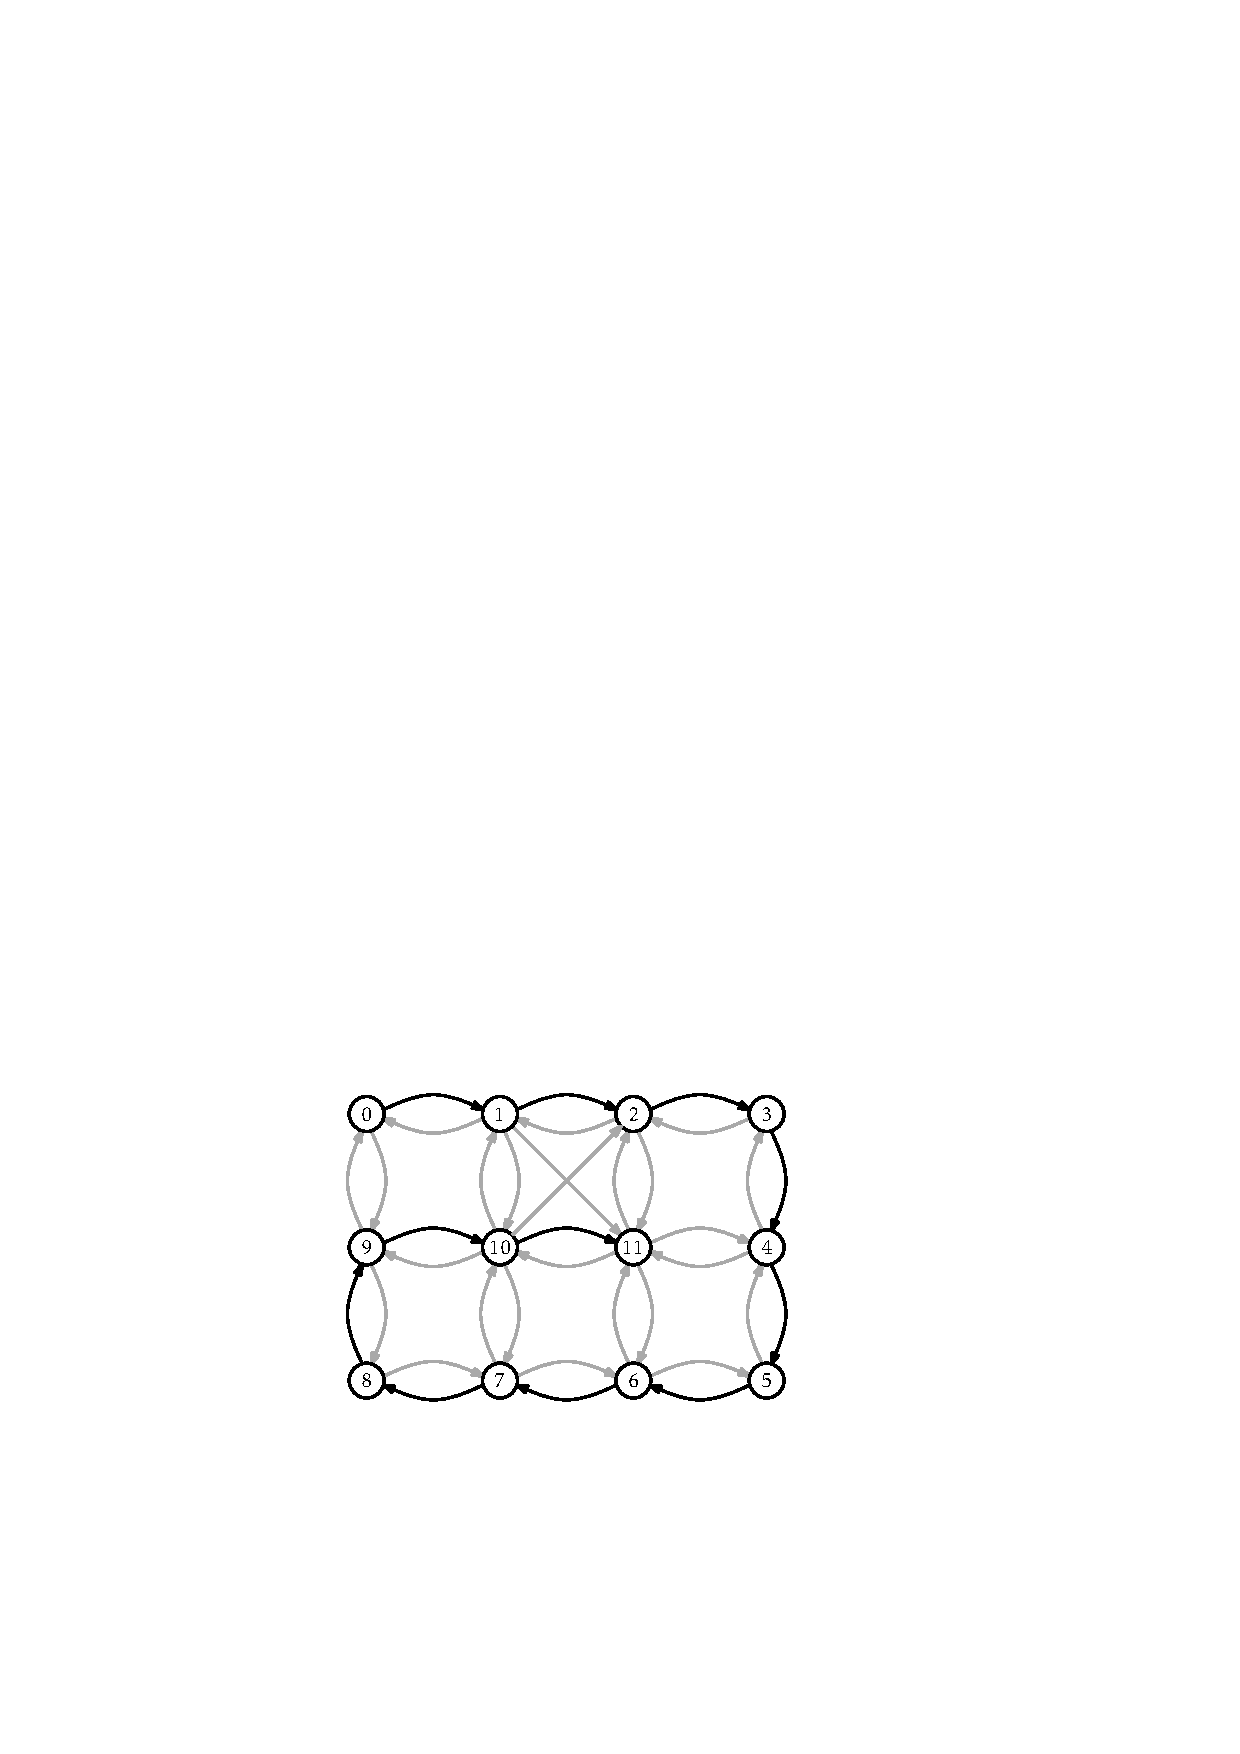
\includegraphics[scale=0.90909]{figs/graph-dfs}
	\end{center}
	\caption[Pesquisa em profundidade]{Um exemplo de pesquisa em profundidade começando no nó 0. Os nós são rotulados com a ordem em que são processados. As arestas que resultam em uma chamada recursiva são desenhadas em preto, outras arestas são desenhadas em #cinza#.}
	\figlabel{graph-dfs}
\end{figure}

Embora a pesquisa em profundidade possa ser melhor considerada um algoritmo recursivo, a recursão não é a melhor maneira de implementá-la. Na verdade, o código fornecido acima falhará para muitos grafos grandes, causando um estouro de pilha. Uma implementação alternativa é substituir a pilha de recursão por uma pilha explícita, #s#. A implementação a seguir faz exatamente isso:
\codeimport{ods/Algorithms.dfs2(g,r)} 
No código anterior, quando o próximo vértice, #i#, é processado, #i# é colorido #cinza# e então substituído, na pilha, por seus vértices adjacentes. Durante a próxima iteração, um desses vértices será visitado.

Não surpreendentemente, os tempos de execução de #dfs(g,r)# e #dfs2(g,r)# são iguais aos de #bfs(g,r)#:
\begin{thm}\thmlabel{dfs-graph}
	Quando dado como entrada um #Grafo#, #g#, que é implementado usando a estrutura de dados #AdjacencyLists#, os algoritmos #dfs(g,r)# e #dfs2(g,r)# são executados em tempo $O(#n#+#m#)$.
\end{thm}

Tal como acontece com o algoritmo de pesquisa em largura, há uma árvore subjacente associada a cada execução da pesquisa em profundidade. Quando um nó $#i#\neq #r#$ vai de #branco# para #cinza#, isso ocorre porque #dfs(g,i,c)# foi chamado recursivamente durante o processamento de algum nó #i'#. (No caso do #dfs2(g,r)# algoritmo, #i# é um dos nós que substituiu #i'# na pilha.) Se pensarmos em #i'# como o pai de #i#, então obtemos uma árvore enraizada em #r#. Em \figref{graph-dfs}, esta árvore é um caminho do vértice 0 ao vértice 11.

Uma propriedade importante do algoritmo de pesquisa em profundidade é a seguinte: Suponha que quando o nó #i# é colorido #cinza#, existe um caminho de #i# para algum outro nó #j# que usa apenas vértices brancos. Então #j# será colorido primeiro #cinza# depois #preto# antes de #i# ser colorido #preto#. (Isso pode ser provado por contradição, considerando qualquer caminho $P$ de #i# a #j#.)

Uma das aplicações desta propriedade é a detecção de ciclos.
\index{detecção de ciclo}%
Consulte a \figref{dfs-cycle}. Considere algum ciclo, $C$, que pode ser alcançado a partir de #r#. Seja #i# o primeiro nó de $C$ colorido #cinza# e seja #j# o nó que precede #i# no ciclo $C$. Então, pela propriedade acima, #j# será colorido #cinza# e a aresta #(j,i)# será considerada pelo algoritmo enquanto #i# ainda é #cinza#. Assim, o algoritmo pode concluir que existe um caminho, $P$, de #i# a #j# na árvore de pesquisa em profundidade e a aresta #(j,i)# existe. Portanto, $P$ também é um ciclo.

\begin{figure}
	\begin{center}
		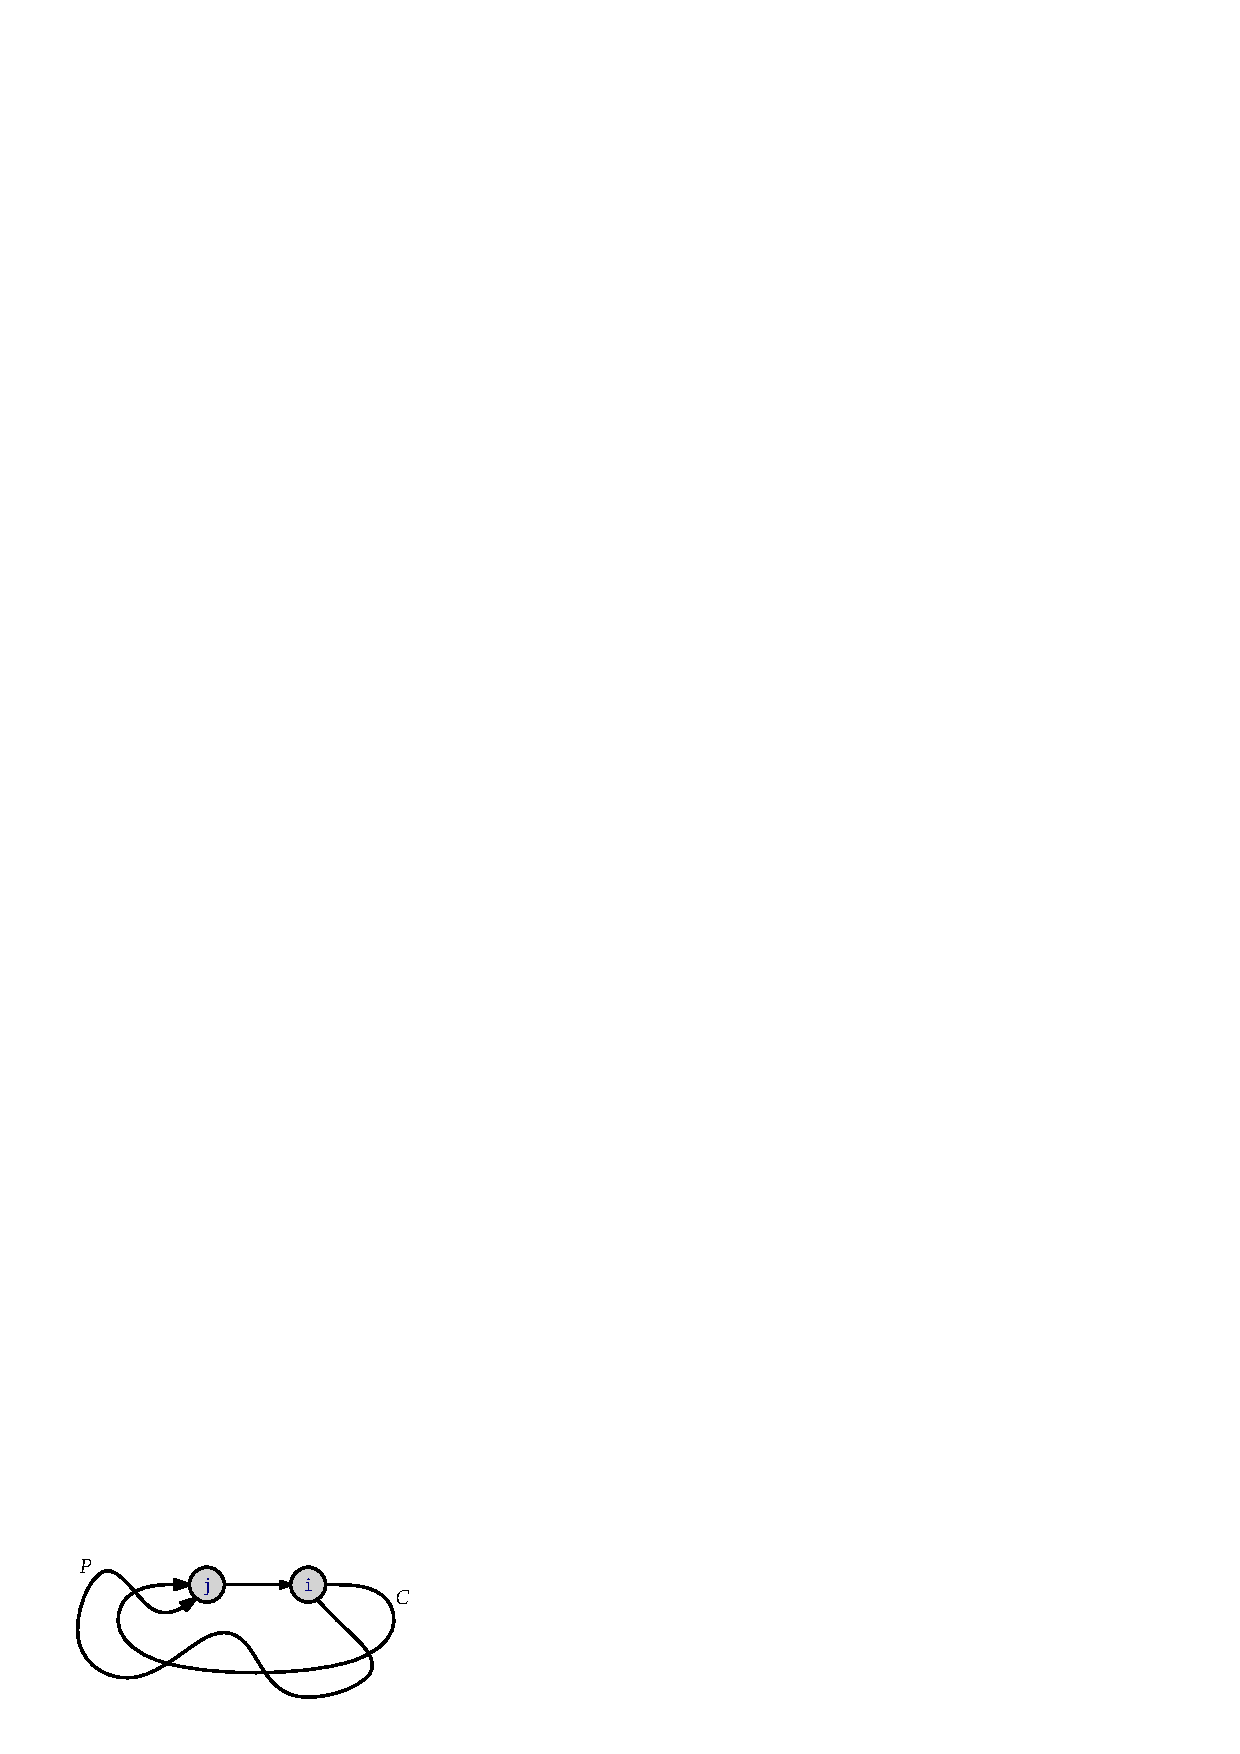
\includegraphics[scale=0.90909]{figs/dfs-cycle}
	\end{center}
	\caption[Detecção de ciclo]{O algoritmo de pesquisa em profundidade pode ser usado para detectar ciclos em $G$. O nó #j# é colorido #cinza# enquanto #i# ainda é #cinza#. Isso implica que há um caminho, $P$, de #i# para #j# na árvore de pesquisa em profundidade, e a aresta #(j,i)# implica que $P$ também é um ciclo.}
	\figlabel{dfs-cycle}
\end{figure}

\section{Discussão e Exercícios}
Os tempos de execução dos algoritmos de pesquisa em profundidade e em largura primeiro são um tanto exagerados pelos Teoremas~\ref{thm:bfs-graph} e \ref{thm:dfs-graph}. Defina $#n#_{#r#}$ como o número de vértices, #i#, de $G$, para os quais existe um caminho de #r# para #i#. Defina $#m#_#r#$ como o número de arestas que têm esses vértices como suas fontes.
Então, o teorema a seguir é uma declaração mais precisa dos tempos de execução dos algoritmos de pesquisa em largura e em profundidade.
(Esta declaração mais refinada do tempo de execução é útil em algumas das aplicações desses algoritmos descritos nos exercícios.)

\begin{thm}\thmlabel{graph-traversal}
	Quando fornecido como entrada um #Grafo#, #g#, que é implementado usando a estrutura de dados #AdjacencyLists#, e algoritmos #bfs(g,r)#, #dfs(g,r)# e #dfs2(g,r)#, cada um executado em tempo $O(#n#_{#r#}+#m#_{#r#})$.
\end{thm}

A pesquisa em largura parece ter sido descoberta independentemente por Moore \cite{m59} e Lee \cite{l61} nos contextos de exploração de labirinto e roteamento de circuito, respectivamente.

As representações de listas de adjacências de grafos foram apresentadas por Hopcroft e Tarjan \cite{ht73} como uma alternativa à (então mais comum) representação de matriz de adjacências. Essa representação, bem como a pesquisa em profundidade, desempenhou um papel importante no famoso algoritmo de teste de planaridade Hopcroft-Tarjan
\index{teste de planaridade}%
que pode determinar, em um tempo $O(#n#)$, se um grafo pode ser desenhado, no plano, e de forma que nenhum par de arestas se cruze \cite{ht74}.

Nos exercícios a seguir, um grafo não direcionado é aquele em que, para cada #i# e #j#, a aresta $(#i#,#j#)$ está presente se e somente se a aresta $(#j#,#i#)$ está presente.
\index{grafo não direcionado}%
\index{grafo!não direcionado}%

\begin{exc}
	Desenhe uma representação de lista de adjacência e uma representação de matriz de adjacência do grafo em \figref{graph-example2}.
\end{exc}

\begin{figure}
	\centering{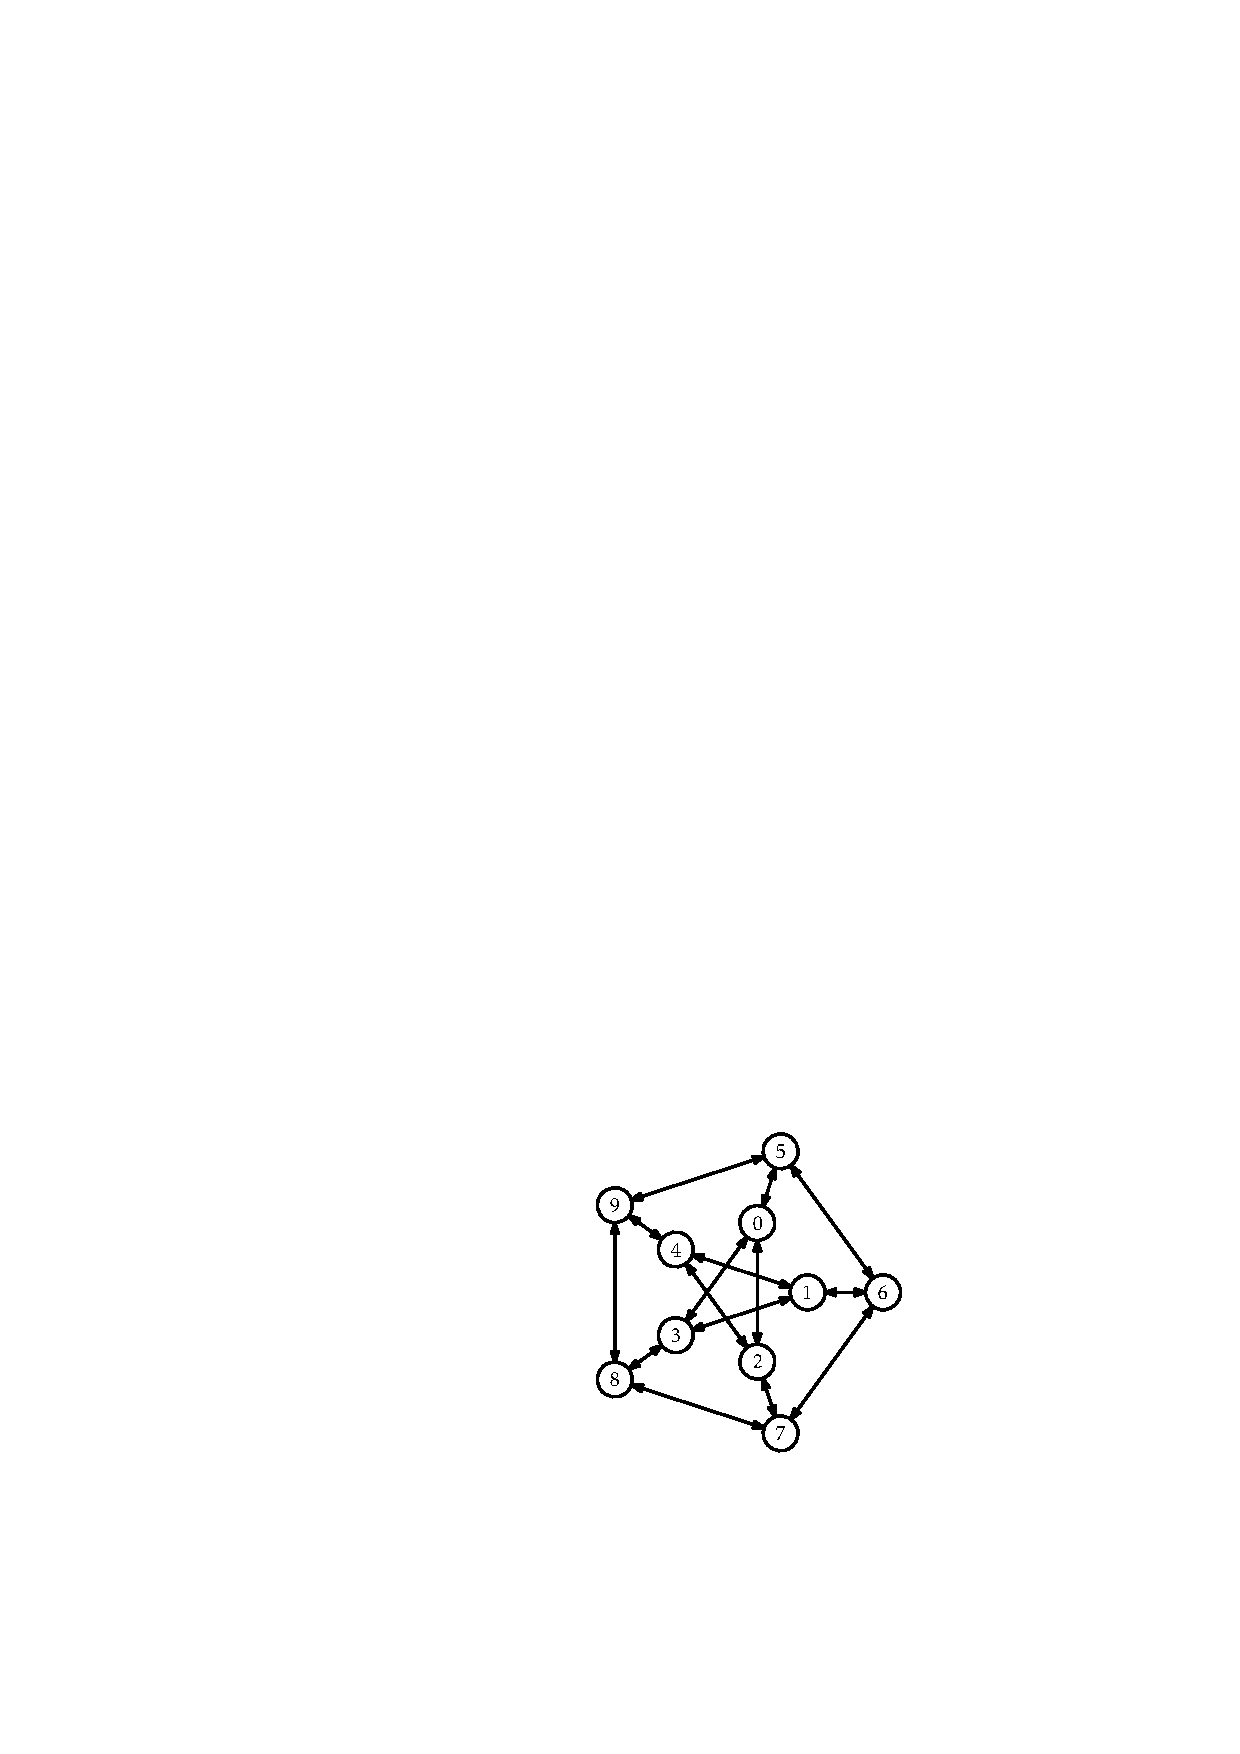
\includegraphics[scale=0.90909]{figs/graph-example2}}
	\caption{Um exemplo de grafo.}
	\figlabel{graph-example2}
\end{figure}

\begin{exc}
	\index{matriz de incidência}%
	A representação \emph{matriz de incidência} de um grafo,
	$G$, é uma $#n#\times#m#$, $A$, onde
	\[
	A_{i,j} = \begin{cases}
	-1 & \text{se o vértice $i$ é a origem da aresta $j$} \\
	+1 & \text{se o vértice $i$ é o alvo da aresta $j$} \\
	0 & \text{caso contrário.}
	\end{cases}
	\]
	\begin{enumerate}
		\item Desenhe a representação da matriz de incidentes do grafo na
		\figref{graph-example2}.
		\item Projetar, analisar e implementar uma representação de matriz de incidência de um grafo. Certifique-se de analisar o espaço, o custo de
		#addEdge(i,j)#, #removeEdge(i,j)#, #hasEdge(i,j)#, #inEdges(i)#,
		e #outEdges(i)#.
	\end{enumerate}
\end{exc}

\begin{exc}
	Ilustre uma execução de #bfs(G,0)# e #dfs(G,0)# no grafo, $#G#$,
	in \figref{graph-example2}.
\end{exc}

\begin{exc}
	\index{grafo conectado}%
	\index{grafo!conectado}%
	Seja $G$ um grafo não direcionado. Dizemos que $G$ é \emph{conectado} se, para cada par de vértices #i# e #j# em $G$, há um caminho de $#i#$ para $#j#$ (uma vez que $G$ é não direcionado, há também um caminho de #j# para #i#). Mostre como testar se $G$ está conectado em um tempo $O(#n#+#m#)$.
\end{exc}

\begin{exc}
	\index{componentes conectados}%
	Seja $G$ um grafo não direcionado. Uma \emph{etiquetagem de componente conectado} de $G$ divide os vértices de $G$ em conjuntos máximos, cada um dos quais forma um subgrafo conectado. Mostre como calcular a etiquetagem de um componente conectado de $G$ em um tempo $ O(#n#+#m#)$.
\end{exc}

\begin{exc}
	\index{floresta extensa}%
	Seja $G$ um grafo não direcionado. Uma \emph{floresta extensa} de $G$ é uma coleção de árvores, uma por componente, cujas arestas são arestas de $G$ e cujos vértices contêm todos os vértices de $G$. Mostre como calcular uma floresta extensa de $G$ em tempo $ O (#n#+#m#) $.
\end{exc}

\begin{exc}
	\index{grafo fortemente conectado}%
	\index{grafo!fortemente conectado}%
	Dizemos que um grafo $G$ é \emph{fortemente conectado} se, para cada par de vértices #i# e #j# em $G$, houver um caminho de $#i#$ para $#j#$. Mostre como testar se $G$ está fortemente conectado em um tempo $O(#n#+#m#)$.
\end{exc}

\begin{exc}
	Dado um grafo $G=(V,A)$ e algum vértice especial $#r#\in V$, mostre como calcular o comprimento do caminho mais curto de $#r#$ a #i# para cada vértice $#i#\in V$.
\end{exc}

\begin{exc}
	Dê um exemplo (simples) em que o código #dfs(g,r)# visita os nós de um grafo em uma ordem diferente daquela do código #dfs2(g,r)#.
	Escreva uma versão de #dfs2(g,r)# que sempre visita os nós exatamente na mesma ordem que #dfs(g,r)#. (Dica: basta começar a rastrear a execução de cada algoritmo em algum grafo onde #r# é a origem de mais de 1 aresta.)
\end{exc}

\begin{exc}
	\index{sumidouro universal}%
	\index{celebridade|see{sumidouro universal}}%
	Um \emph{sumidouro universal} em um grafo $G$ é um vértice que é o alvo de $#n#-1$ arestas e a fonte de nenhuma aresta.\footnote{Um sumidouro universal, #v#, também é às vezes chamado de \emph{celebridade}: todos na sala reconhecem #v#, mas #v# não reconhece ninguém na sala.}
	Projete e implemente um algoritmo que testa se um grafo $G$, representado como #AdjacencyMatrix#, tem um sumidouro universal. Seu algoritmo deve ser executado em tempo $O(#n#)$.
\end{exc}


